\begin{center}
\makeatletter
\@ifundefined{color@atlasink}{\definecolor{atlasink}{HTML}{33312E}}{}
\@ifundefined{color@atlasgray}{\definecolor{atlasgray}{HTML}{9A958C}}{}
\@ifundefined{color@atlasblue}{\definecolor{atlasblue}{HTML}{2E6F9E}}{}
\@ifundefined{color@atlasgreen}{\definecolor{atlasgreen}{HTML}{4C8C3F}}{}
\@ifundefined{color@atlasred}{\definecolor{atlasred}{HTML}{C0473B}}{}
\@ifundefined{color@atlasgold}{\definecolor{atlasgold}{HTML}{D69A2A}}{}
\@ifundefined{atlascaption}{%
  \newcommand{\atlascaption}[3]{\shortstack{\footnotesize Figure~#1. \textbf{#2:}\\#3}}%
}{}
\@ifundefined{glowstroke}{%
  \newcommand{\glowstroke}[3]{%
    \draw[#1, line width=1.5pt, line cap=round]
      plot[domain=#2,samples=100,smooth] (\x,{#3});%
  }%
}{}
\makeatother
\tikzset{
  atlas axes/.style={atlasink, line width=0.7pt, line cap=round, ->},
  atlas curve/.style={line width=1.5pt, line cap=round, line join=round},
  dropline/.style={atlasgray, line width=0.6pt, dash pattern=on 2pt off 2pt},
  atlas dot/.style={fill=atlasink, draw=white, line width=0.4pt, circle, inner sep=0pt, minimum size=4.2pt},
}

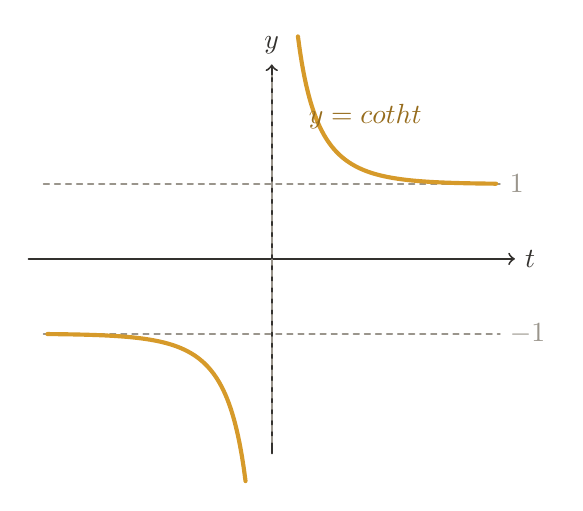
\begin{tikzpicture}[scale=0.95, line cap=round, line join=round]
  \draw[atlas axes] (-3.25,0)--(3.25,0) node[right] {$t$};
  \draw[atlas axes] (0,-2.6)--(0,2.6) node[above] {$y$};
  \draw[dropline] (-3.05,1)--(3.05,1) node[right] {$1$};
  \draw[dropline] (-3.05,-1)--(3.05,-1) node[right] {$-1$};
  \draw[dropline] (0,-2.45)--(0,2.45);
  \glowstroke{atlasgold}{0.35:3}{(exp(\x)+exp(-\x))/(exp(\x)-exp(-\x))}
  \glowstroke{atlasgold}{-3:-0.35}{(exp(\x)+exp(-\x))/(exp(\x)-exp(-\x))}
  \node[atlasgold!70!black] at (1.25,1.9) {$y=\operatorname{coth}t$};
\end{tikzpicture}

\atlascaption{H5}{Hyperbolic cotangent}{Undefined at $t=0$, with asymptotes $y=\pm 1$.}
\end{center}
